\documentclass[spanish]{beamer}

%%% CODIFICACIÓN

%\usepackage[x11names, rgb, html]{xcolor}
\usepackage[utf8]{inputenc}
\usepackage[spanish]{babel}
\usepackage{graphics}

%%% FUENTES

\usepackage[T1]{fontenc}
%\usepackage[familydefault,regular]{Chivo}
%\usepackage{newtxsf} % Fuente de matemáticas
%\usepackage{mathastext}
%\usepackage[scaled=.85]{FiraMono}

\setbeamertemplate{navigation symbols}{}

%%% COLORES

\definecolor{50}{HTML}{FFEBEE}
\definecolor{100}{HTML}{FFCDD2}
\definecolor{200}{HTML}{EF9A9A}
\definecolor{300}{HTML}{E57373}
\definecolor{400}{HTML}{EF5350}
\definecolor{500}{HTML}{F44336}
\definecolor{600}{HTML}{E53935}
\definecolor{700}{HTML}{D32F2F}
\definecolor{800}{HTML}{C62828}
\definecolor{900}{HTML}{B71C1C}

%% Colores de Solarized

\definecolor{sbase03}{HTML}{002B36}
\definecolor{sbase02}{HTML}{073642}
\definecolor{sbase01}{HTML}{586E75}
\definecolor{sbase00}{HTML}{657B83}
\definecolor{sbase0}{HTML}{839496}
\definecolor{sbase1}{HTML}{93A1A1}
\definecolor{sbase2}{HTML}{EEE8D5}
\definecolor{sbase3}{HTML}{FDF6E3}
\definecolor{syellow}{HTML}{B58900}
\definecolor{sorange}{HTML}{CB4B16}
\definecolor{sred}{HTML}{DC322F}
\definecolor{smagenta}{HTML}{D33682}
\definecolor{sviolet}{HTML}{6C71C4}
\definecolor{sblue}{HTML}{268BD2}
\definecolor{scyan}{HTML}{2AA198}
\definecolor{sgreen}{HTML}{859900}

%% Colores del documento

\definecolor{background}{RGB}{237,237,237}
\definecolor{text}{RGB}{78,78,78}
\definecolor{accent}{RGB}{129, 26, 24}
\definecolor{accent2}{HTML}{814918}
\definecolor{accent3}{HTML}{136618}
\definecolor{accent4}{HTML}{0F4B4E}
\definecolor{accent5}{HTML}{681341}
\definecolor{accent6}{HTML}{1F1B5A}

\setbeamerfont{framesubtitle}{size=\normalfont\small}
\setbeamercolor{framesubtitle}{fg=white}

%%% AJUSTES DE BEAMER

% ¿Negrita en el título de diapositiva o no?
%\setbeamertemplate{frametitle}{\color{accent}\vspace*{1cm}\bfseries\insertframetitle\par\vskip-6pt}

\setbeamertemplate{frametitle}{\color{900}\vspace*{1cm}\insertframetitle\\\usebeamerfont{framesubtitle}\insertframesubtitle\par\vskip-6pt}

\setbeamertemplate{itemize items}[circle] % Viñetas de itemize

%%% CONFIGURACIÓN DE COLORES DE BEAMER

\setbeamercolor{background canvas}{bg=background}
\setbeamercolor{normal text}{fg=text}
\setbeamercolor{alerted text}{fg=900}
\setbeamercolor{block title}{fg=900}
\setbeamercolor{alerted text}{fg=900}
\setbeamercolor{itemize item}{fg=900}
\setbeamercolor{enumerate item}{fg=900}
\setbeamercolor*{title}{fg=900}
\setbeamercolor{qed symbol}{fg=900}
\usebeamercolor[fg]{normal text}

%%% INFORMACIÓN DEL DOCUMENTO

\title{Fundamentos de Redes}
\subtitle{Redes anónimas: I2P}
\author{Alberto Jesús Durán López\\ Antonio Coín Castro\\ \vspace{1em}Grupo 5}
\begin{document}


\maketitle

%%% Inicio diapositiva
\begin{frame}{Anonimato en el acceso corriente a internet}%{Subtítulo (opcional)}

Hableremos sobre distintas formas de obtener anonimato: \\ %Puedes comentar esta línea si quieres

\vspace{1.5em} %% espaciado vertical

\begin{itemize}
	\item Proxy, VPN...
    \item I2P, Invisible Internet Project \\ 
\end{itemize}

\vspace{1.5em} %% espaciado vertical

%El espaciado vertical se controla con "$\textbackslash$vspace$\{1.2em\}$", modificando el número de dentro.

\end{frame}  
%%% Fin diapositiva





\begin{frame}
	Podemos poner una diapos. con una foto introductoria para el simil de cuando
	nos conectamos a la red - plaza , if u want it would be great
\end{frame}







\begin{frame}{Métodos para mantener el anonimato}
	
\begin{itemize}
	\item Proxy \\
	\item VPN - Virtual Private Network \\ 
	\item Otros
\end{itemize}	
	
	
\end{frame}






\begin{frame}{Proxy}
	
Servidor intermediario entre las conexiones de un cliente y un servidor. \\


\begin{figure}[h]
	\centering
	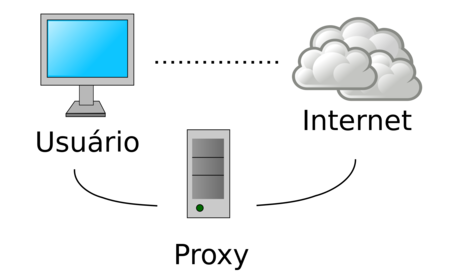
\includegraphics[width=.5\textwidth]{img/proxy}
\end{figure}

\begin{itemize}
	\item Dirección IP camuflada \\
	\item Acceso a contenido bloqueados de algunos países \\ 
\end{itemize}
	
\end{frame}




\begin{frame}{VPN}
	\begin{figure}[h]
		\centering
		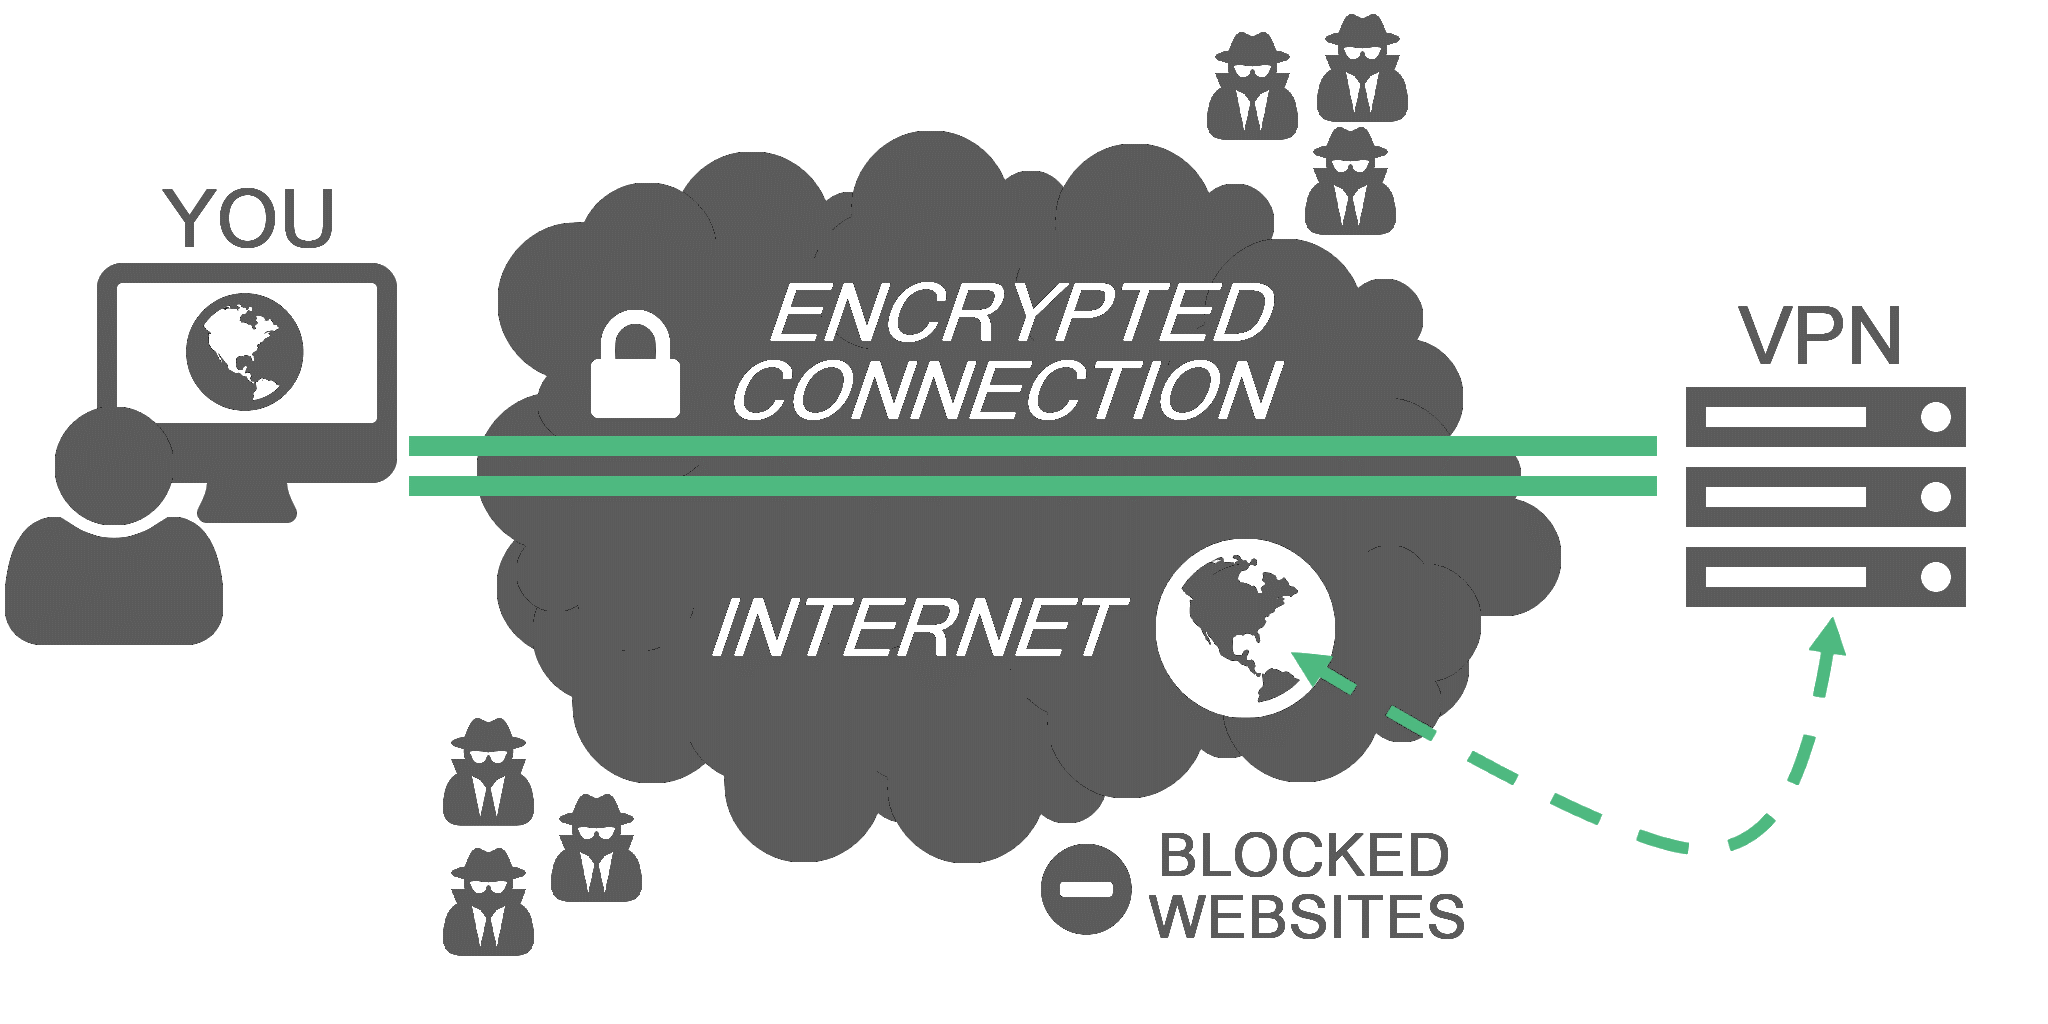
\includegraphics[width=.8\textwidth]{img/vpn}
	\end{figure}
\end{frame}



\begin{frame}{VPN}

Medio de extender una red privada a través de una red pública

\vspace{1.9em}

\begin{itemize}
	\item Se puede acceder a una red privada remotamente \\
	\item Dirección IP camuflada \\ 
	\item Confidencialidad garantizada - Paquetes encriptados \\
	\item Sistema de autentificación para conectarse
	\item Mecanismos para mantener integridad de mensajes
\end{itemize}	

\end{frame}






\begin{frame}{Otros...}

\begin{itemize}
	\item Tails % Sistema operativo pensado en la seguridad
	\item DuckDuckGo
\end{itemize}

\begin{figure}[h]
	\centering
	%
\includegraphics[width=.3\textwidth]{img/duck} %No queda muy bien, no? 
\end{figure}

\end{frame}



\begin{frame}{I2P, Invisible Internet Project}
	
Se puede poner diapositiva introductoria a I2P con foto	
	
\end{frame}




\begin{frame}{I2P, Invisible Internet Project}
	
	
\begin{itemize}
	\item Nodos y túneles
	\item Enrutamiento tipo garlic
	\item Encriptación de la información
\end{itemize}	
	
\end{frame}






\begin{frame}{I2P, Invisible Internet Project}
	
	Nodos y túneles for you
	and kademlia too	
	
\end{frame}






\begin{frame}{Enrutamiento tipo garlic}
	


\begin{itemize}
	\item Cifrado por capas
	\item Agregación de múltiples mensajes juntos
	\item Cifrado ElGamal/AES
\end{itemize}
	
	
\end{frame}







\begin{frame}{Enrutamiento tipo garlic}

Cifrado por capas:


\begin{itemize}
	\item Comunicación de dos usuarios mediante túneles
	\item La información viaja desde el primer nodo del túnel hasta el último
	\item El 'gateway' fragmenta mensajes I2P en mensajes de túnel
	\item En cada salto se envía: \{ID del túnel, IV, mensaje del túnel\}
\end{itemize}


\end{frame}


\begin{frame}{Enrutamiento tipo garlic}


Agregación de múltiples mensajes juntos juntos para aumentar velocidad de transferencia de datos y aumentar seguridad
	
%Se puede poner alguna foto para acompañar
	
\end{frame}



\begin{frame}{Enrutamiento tipo garlic}
	Mensajes cifrados usando ElGamal/AES
\end{frame}



\begin{frame}{Encriptación de la información}

\begin{itemize}
	\item ElGamal
	\item AES: Cifrado simétrico por bloques de 128 bits
	\item Procedimiento aplicado a los mensajes:
	\begin{itemize}
		\item Se cifra el IV recibido con AES
		\item Usa el IV obtenido para cifrar los datos
		\item Cifra de nuevo el IV usando AES
		\item Envía \{ID del túnel, IV, mensaje del túnel\} al siguiente nodo
	\end{itemize}
\end{itemize}



\end{frame}



\begin{frame}{Software I2P}
	

\begin{itemize}
	\item Susimail: Interfaz web  para emails
	\item Syndie: blogs, noticias y foros para I2P
	\item I2P Messenger: Cliente de mensajería instantánea
	\item Navegación web mediante webs anónimas
	\item Compartición de archivos mediante el uso de BitTorrent dentro de la red I2P
	\item (Android) Nightweb, aplicación que usa I2P y BitTorrent para compartir entradas
	de blogs, fotos y otros contenidos similares
\end{itemize}
	
\end{frame}











\end{document}
